\documentclass[12pt, a4paper]{article}
\usepackage[utf8]{inputenc}
\usepackage[russian]{babel}
\usepackage[pdftex]{graphicx, color}
\usepackage[left=2cm,right=2cm,top=1.5cm,bottom=2cm]{geometry}
\usepackage{indentfirst}
\usepackage{float}
\usepackage{hyperref}
\usepackage[justification=centering]{caption}
\usepackage{amsmath, amsfonts, amssymb, amsthm, amsbsy, mathtools}

\usepackage{setspace}
\onehalfspacing
\graphicspath{{pics/}}

\begin{document}
    \begin{singlespace}
    \begin{center}
        
\includegraphics[height=3cm]{msu.png}

        {\large\textbf{Отчёт по практической работе по курсу ГО\\
        <<Автоматическое дифференцирование для автокодировщика>>}}

        \vspace{0.3cm}

        \textit{\textbf{Аят Оспанов}}

        617 гр., ММП, ВМК МГУ, Москва

        12 октября 2017 г.
    \end{center}
    \end{singlespace}

    \tableofcontents

    \section{Модель автокодировщика}
        Для задания модели автокодировщика рассмотрим сначала полносвязный слой нейронной сети, показанный на рис. \ref{fig:net}, слева. Данный слой принимает на вход вектор $x \in \mathbb{R}^p$ размерности $p$ и возвращает вектор $z \in \mathbb{R}^q$ размерности $q$. При этом каждый выходной элемент (нейрон) $z_i$ вычисляется с помощью 1) линейной комбинации входящих в него элементов $x_j$ с весами $w_{ij}$ c добавлением сдвига $b_i$ и 2) применения к результату линейной комбинации некоторой одномерной нелинейной функции активации $g$:
        $$\boldsymbol{z} = g(W\boldsymbol{x} + \boldsymbol{b}) = g(\overline{W}\overline{\boldsymbol{x}}) \text{,}$$
        где $W \in \mathbb{R}^{q\times p}$, $\boldsymbol{b} \in \mathbb{R}^q$ и $\overline{W} = [W, \boldsymbol{b}]$, $\overline{\boldsymbol{x}} = [\boldsymbol{x}^T, 1]^T$ -- расширенные матрица весов и вектор входа. В качестве операции $g$ может использоваться как тождественное преобразование, так и простая нелинейная функция.

        Модель автокодировщика состоит из нескольких полносвязных слоёв (см. рис. \ref{fig:net}, справа). Входной и выходной слои состоят из $D$ нейронов, симметричные скрытые слои имеют одинаковое число нейронов, а средний слой состоит из $d$ нейронов. Обозначим через $\boldsymbol{z}^l$ выход $l$-го скрытого слоя, где $l = 0, 1, 2, \dots, L, \boldsymbol{z}^0 = \boldsymbol{x}; \boldsymbol{z}^L$ -- выход последнего слоя. Обучение автокодировщика осуществляется путём решения следующей задачи оптимизации:
        $$F(\boldsymbol{\theta})=\frac{1}{n}\sum\limits_{i=1}^{n} L(\boldsymbol{x}_i, z^L(\boldsymbol{x}_i, \boldsymbol{\theta})) \rightarrow \min_\theta$$
        Здесь в качестве функции потерь выступает $L(\boldsymbol{x},\boldsymbol{z}) = \frac{1}{2}\lVert\boldsymbol{x}-\boldsymbol{z}\rVert^2$, а через $\boldsymbol{\theta}$ обозначены параметры всех скрытых слоёв $\{W_l\}_{l=1}^L$

        \begin{figure}
            \centering
            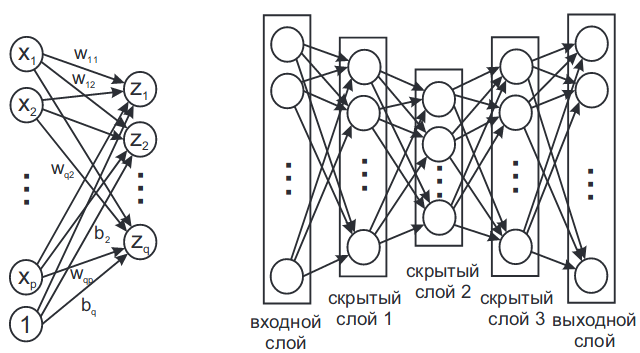
\includegraphics[width=0.8\linewidth]{net}
            \caption{Пример автокодировщика с тремя скрытыми слоями}
            \label{fig:net}
        \end{figure}

    \section{Вычисление произведения гессиана на вектор: $R_p$ проход назад}
        Все величины для $R_p$ прохода назад вычисляются применением оператора $R_p\{\cdot\}$ к каждой строчке алгортима прохода назад. В итоге получаем следующий алгоритм:
        \begin{gather}
        \begin{align*}
            R_p&\{\nabla_{\boldsymbol{z}^L}L\} = R_p\{\boldsymbol{z}^L - x\} = R_p\{\boldsymbol{z}^L\}\\
            R_p&\{\nabla_{\boldsymbol{u}^L}L\} = R_p\{\nabla_{\boldsymbol{z}^L}L\} \odot g'(\boldsymbol{u}^L) + \nabla_{\boldsymbol{z}^L}L \odot g''(\boldsymbol{u}^L) \odot R_p\{\boldsymbol{u}^L\}\\
            R_p&\{\nabla_{\overline{W}^L}L\} = R_p\{\nabla_{\boldsymbol{u}^L}L\} (\overline{\boldsymbol{z}}^{L-1})^T + (\nabla_{\boldsymbol{u}^L}L) R_p\{\overline{\boldsymbol{z}}^{L-1}\}^T\\
            \textbf{дл}&\textbf{я } l = L-1, L-2, \dots, 1\text{:}\\
            &R_p\{\nabla_{\boldsymbol{z}^l}L\} = (P^{l+1})^T \nabla_{\boldsymbol{u}^{l+1}}L + (W^{l+1})^T R_p\{\nabla_{\boldsymbol{u}^{l+1}}L\}\\
            &R_p\{\nabla_{\boldsymbol{u}^l}L\} = R_p\{\nabla_{\boldsymbol{z}^l}L\} \odot g'(\boldsymbol{u}^l) + \nabla_{\boldsymbol{z}^l}L \odot g''(\boldsymbol{u}^l) \odot R_p\{\boldsymbol{u}^l\}\\
            &R_p\{\nabla_{\overline{W}^l}L\} = R_p\{\nabla_{\boldsymbol{u}^l}L\} (\overline{\boldsymbol{z}}^{l-1})^T + (\nabla_{\boldsymbol{u}^l}L) R_p\{\overline{\boldsymbol{z}}^{l-1}\}^T
        \end{align*}
        \end{gather}

    \section{Исследования}
        \subsection{Вычисление $\nabla F(\boldsymbol{\theta})$ и $\nabla^2 F(\boldsymbol{\theta}) \boldsymbol{p}$}
            В процессе исследований модели автокодировщика были проверены корректность вычислений градиента функции потерь, гессиана на вектор и Гаусс-Ньютоновской аппроксимации гессиана на вектор. Сравнение значений с помощью разностных аппроксимаций показывает следующие результаты:
            \begin{itemize}
                \item Градиент функции потерь считается с точностью до $10^{-14}$: косинусное расстояние от численно высчитанного градиента до градиента, полученного автокодировщиком равняется 1
                \item Гессиан функции потерь умноженный на вектор считается с точностью до $10^{-14}$: косинусное расстояние от численно высчитанного произведения до произведения, полученного автокодировщиком равняется 1
                \item Гаусс-Ньютоновская аппроксимация гессиана функции потерь умноженная на вектор считается не точно: косинусное расстояние от численно высчитанного произведения до произведения, полученного автокодировщиком равняется 0.6
            \end{itemize}

        \subsection{Стохастические методы оптимизации}
            В качестве набора данных был взят MNIST. Данные были отнормированы на отрезок $[0, 1]$. Были исследованы три архитектуры автокодировщика:
            \begin{itemize}
                \item 3 слоя: вход - 2 нейрона - выход
                \item 5 слоев: вход - 200 - 2 - 200 - выход
                \item 7 слоев: вход - 400 - 200 - 2 - 200 - 400 - выход
            \end{itemize}

            Во всех архитектурах: центральный слой имеет линейную функцию активации, последний слой -- сигмоиду, остальные -- ReLU/LeakyReLU. Во всех слоях, кроме последнего используется сдвиг. Для каждого метода было сделано 33 итераций. В итоге получились следующие результаты:

            \begin{figure}[p]
                \centering
                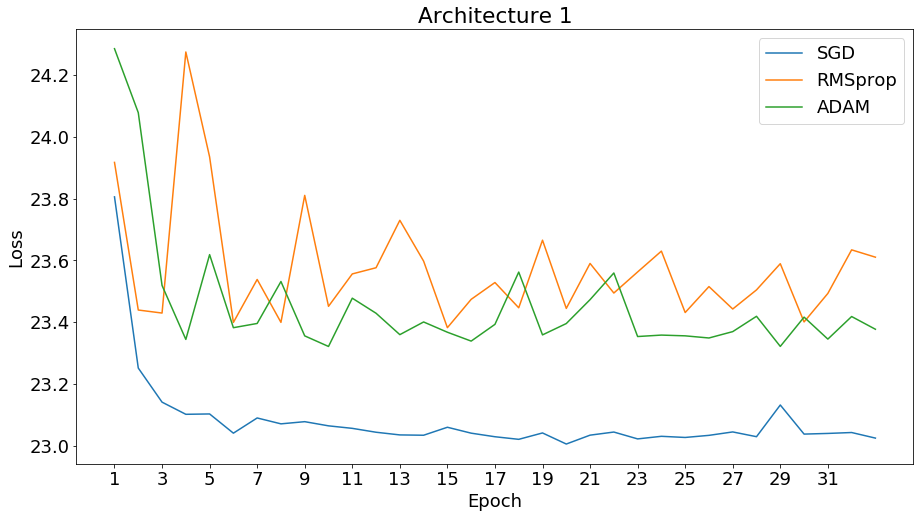
\includegraphics[width=0.7\linewidth]{pics/arch1_loss}
                \caption{График сходимости для первой архитектуры на тестовых данных}
                \label{fig:arch1_loss}
            \end{figure}

            Из графика \ref{fig:arch1_loss} видно, что методы оптимизации ведут себя не стабильно. Это скорее всего связано с тем, что модель резко сжимает пространство (с 784 до 2), что приводит к неустойчивости.

            \begin{figure}[p]
                \centering
                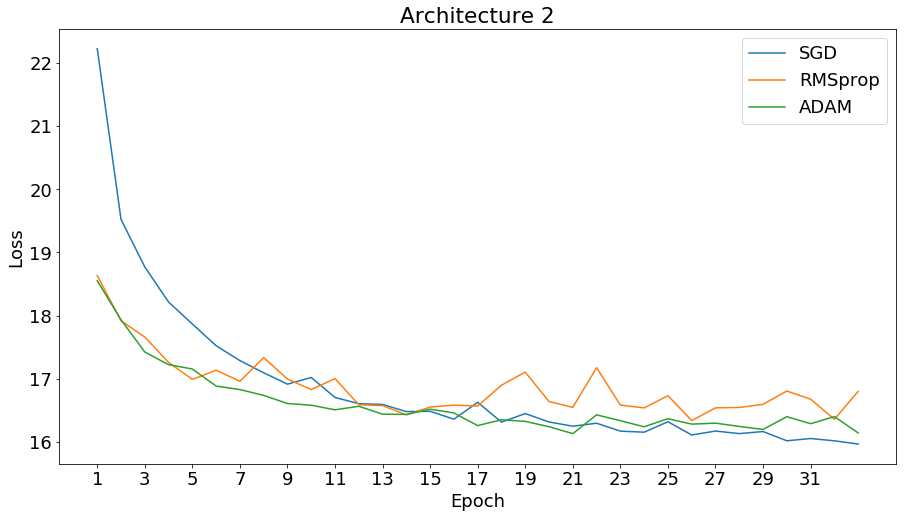
\includegraphics[width=0.7\linewidth]{pics/arch2_loss}
                \caption{График сходимости для второй архитектуры на тестовых данных}
                \label{fig:arch2_loss}
            \end{figure}

            В графике \ref{fig:arch2_loss} видно, что в этой архитектуре методы оптимизации работают корректно. Также видно, что они работают примерно одинаково, но метод ADAM сходится быстрее.

            \begin{figure}[p]
                \centering
                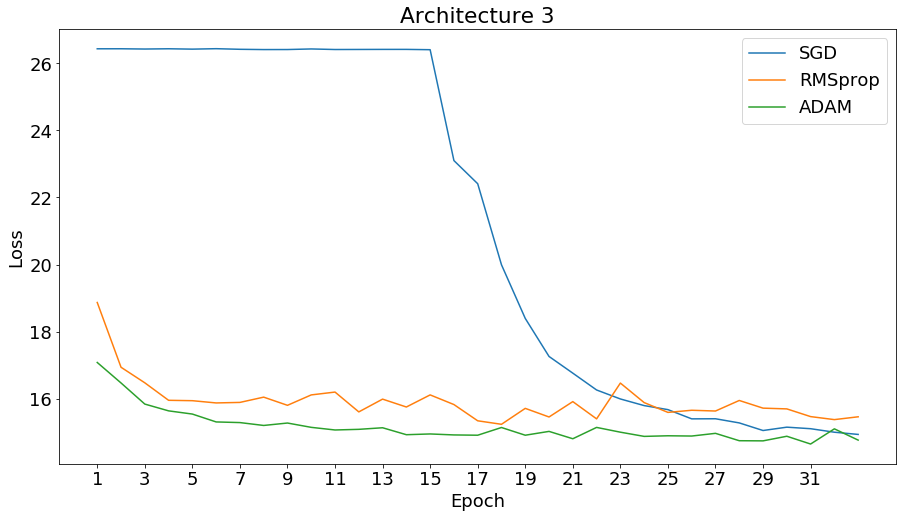
\includegraphics[width=0.7\linewidth]{pics/arch3_loss}
                \caption{График сходимости для третьей архитектуры на тестовых данных}
                \label{fig:arch3_loss}
            \end{figure}

            В третьей архитектуре (Рис. \ref{fig:arch3_loss}) метод SGD повел себя странно. И начал существенно сходится только с 16 эпохи, но к концу теста все же сошелся к другим методам. В этом случае так же ADAM сходится быстрее и ведет себя устойчиво. Также была замечена тенденция, что при больших количествах слоев, метод SGD настраивается не сразу, а спустя несколько эпох.

            В таблице \ref{tab:io} можно посмотреть как обучились автокодировщики. В случае с первой архитектурой выход является нечетким, т.к. методы не сошлись за отведенное количество итераций. Архитектуры 2 и 3 оптимизировались хорошо. Также видно, что методы SGD и ADAM сработали лучше для второй архитектуры, а ADAM и RMSprop -- для третьей архитектуры. Учитывая все результаты, можно сделать вывод, что ADAM работает лучше других стохастических методов оптимизаций.

            \begin{table}\caption{Входы и выходы сетей}
            \label{tab:io}
            \begin{tabular}{c c c}
                \textbf{Архитектура 1} & \textbf{Архитектура 2} & \textbf{Архитектура 3}\\
                % \hline
                \multicolumn{3}{c}{\textbf{SGD}}\\
                % \hline
                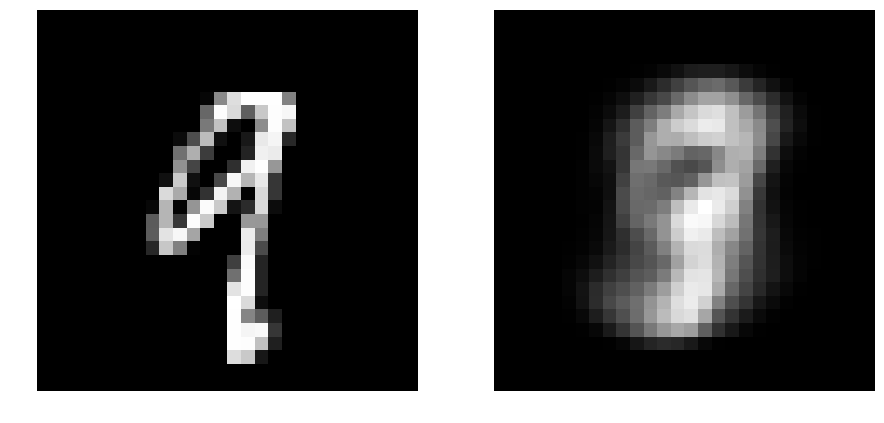
\includegraphics[width=0.3\linewidth]{pics/arch1_sgd} &
                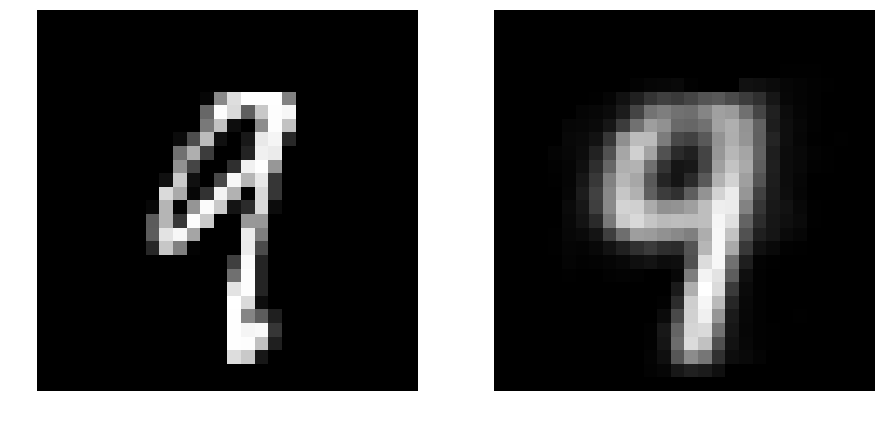
\includegraphics[width=0.3\linewidth]{pics/arch2_sgd} &
                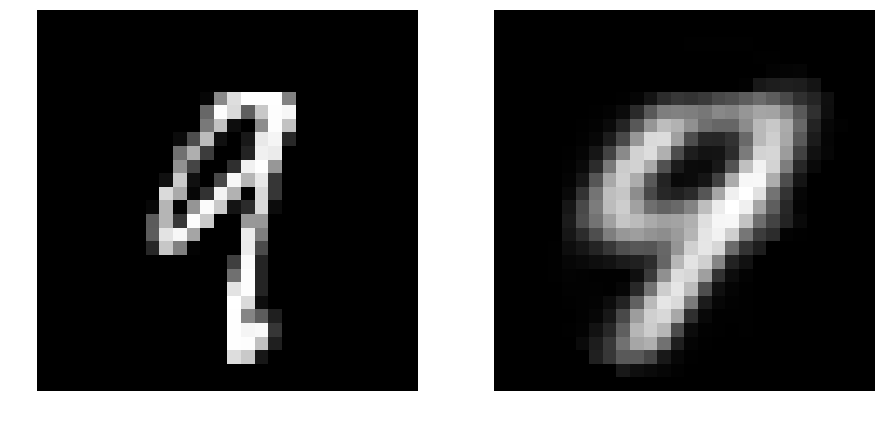
\includegraphics[width=0.3\linewidth]{pics/arch3_sgd} \\
                % \hline
                \multicolumn{3}{c}{\textbf{RMSprop}}\\
                % \hline
                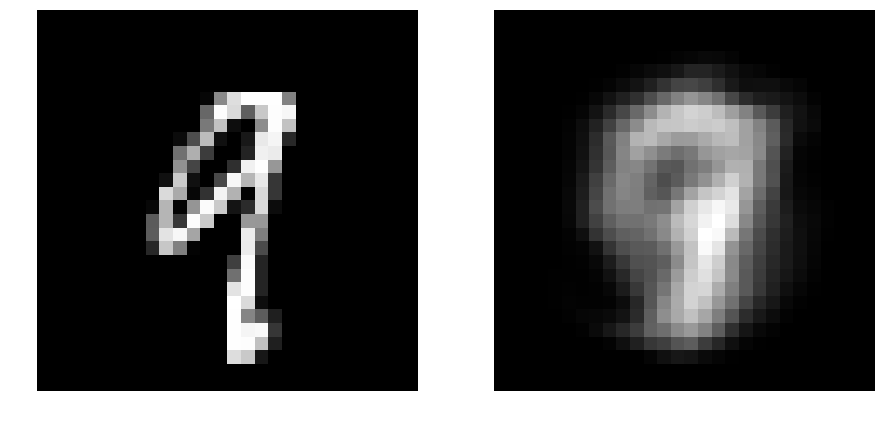
\includegraphics[width=0.3\linewidth]{pics/arch1_rmsprop} &
                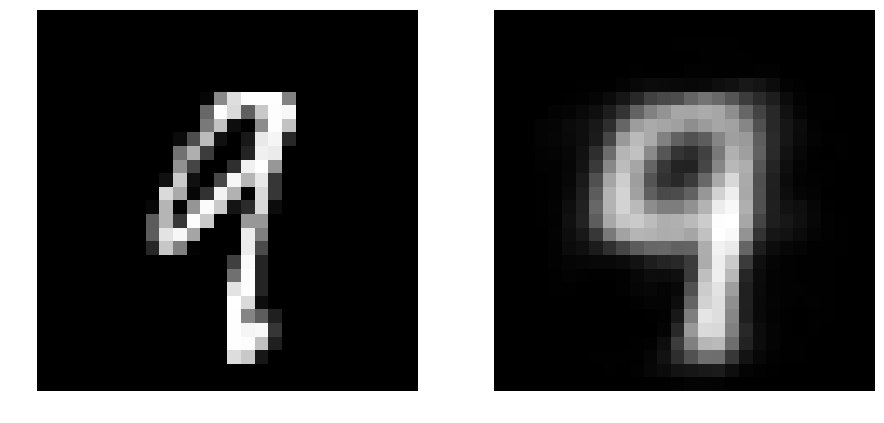
\includegraphics[width=0.3\linewidth]{pics/arch2_rmsprop} &
                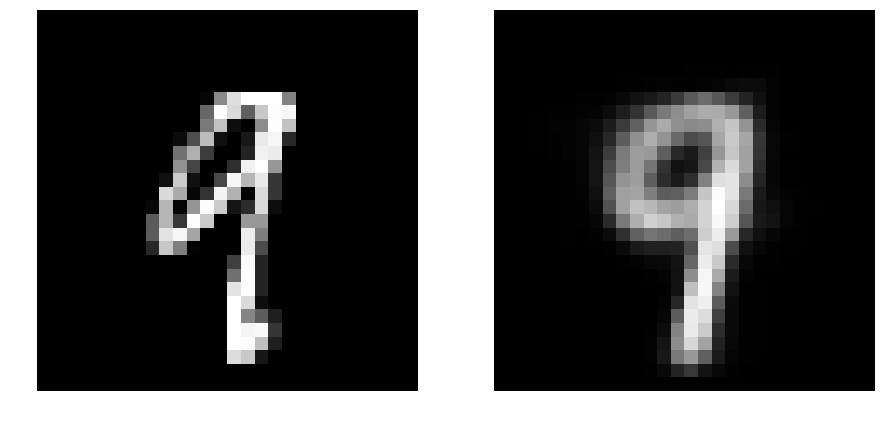
\includegraphics[width=0.3\linewidth]{pics/arch3_rmsprop} \\
                % \hline
                \multicolumn{3}{c}{\textbf{ADAM}}\\
                % \hline
                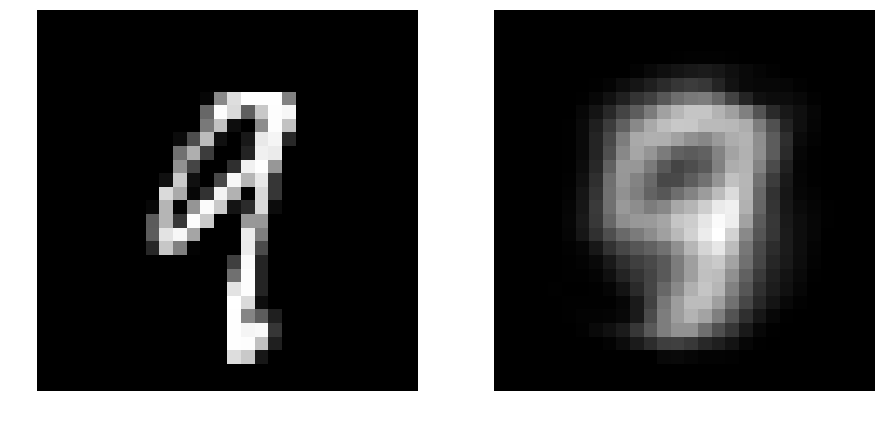
\includegraphics[width=0.3\linewidth]{pics/arch1_adam} &
                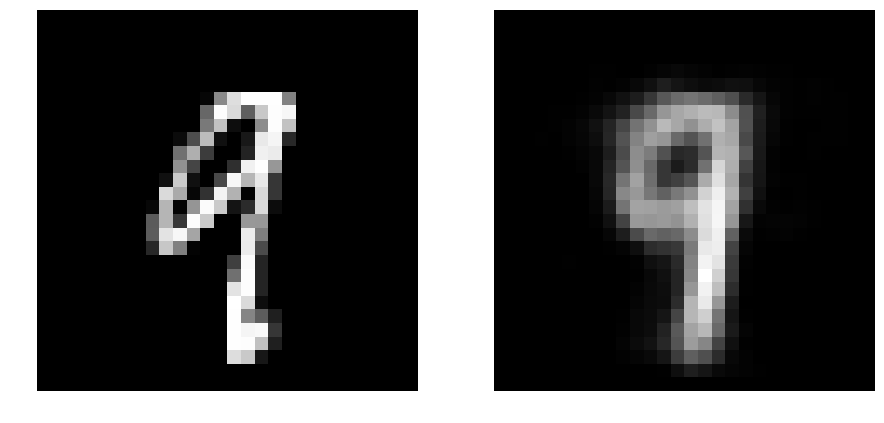
\includegraphics[width=0.3\linewidth]{pics/arch2_adam} &
                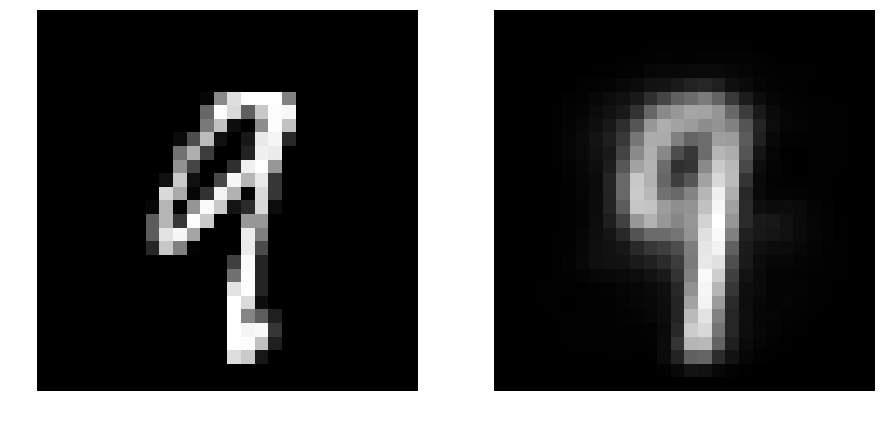
\includegraphics[width=0.3\linewidth]{pics/arch3_adam} \\
            \end{tabular}
            \end{table}

        \subsection{Подбор параметров}
            Подбор параметров велся обычной сеткой на 2ой архитектуре автокодировщика с использованием метода ADAM. Подбирались независимо длина шага и количество мини-батчей. В итоге получились следующие графики:
            \begin{figure}[h]
                \centering
                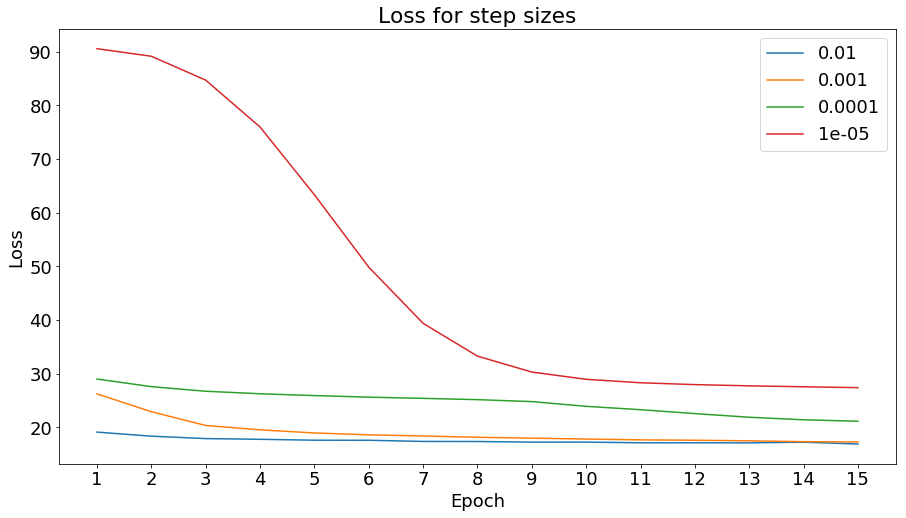
\includegraphics[width=0.49\linewidth]{pics/loss_step}
                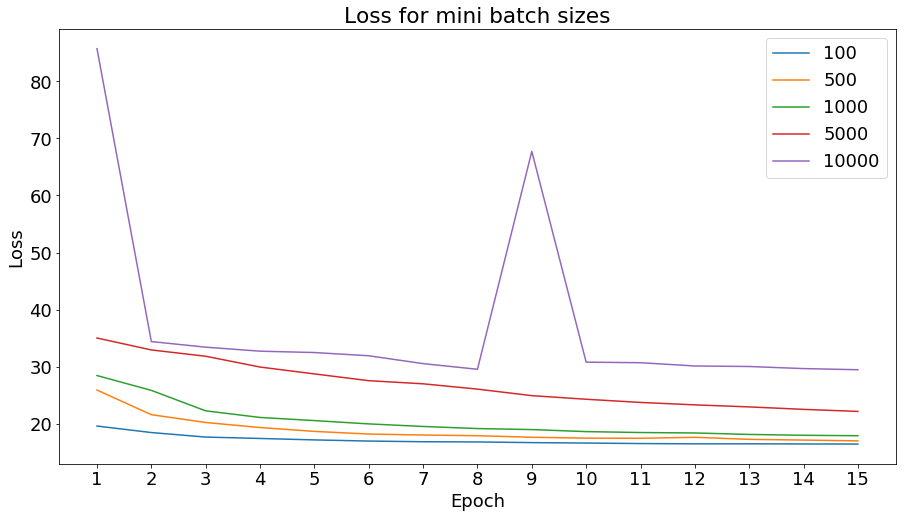
\includegraphics[width=0.49\linewidth]{pics/loss_batch}
                \caption{График сходимости для разных длин шагов (слева) и для разных размеров мини-батчей (справа)}
                \label{fig:params}
            \end{figure}

        Из графиков можно понять, что длина шага 0.01 и размер батчей в 100 элементов являются оптимальными. Также видно, что чем больше количество батчей, тем медленнее сходитя метод. На 10000 батчей даже видно подскок в значении функции потерь. Похожая ситуация с шагом метода. Чем ближе шаг в 0.01, тем быстрее метод сходится. Более точный анализ значений не требуется, т.к. размер шага в маленькой окрестности 0.01 не особо повлияет на скорость сходимости, как и количество батчей.

        \subsection{Визуализация}
            Попробуем нарисовать выход среднего слоя в 2 нейрона и раскрасить их в цвета своих классов.
            \begin{figure}[h]
                \centering
                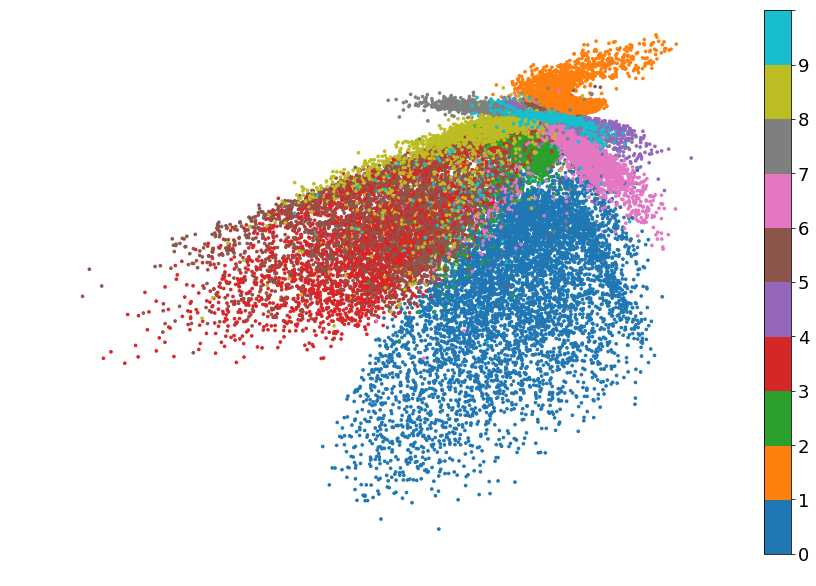
\includegraphics[width=\linewidth]{pics/2dim}
                \caption{Визуализация объектов MNIST}
                \label{fig:2dim}
            \end{figure}

            Четко видно, что объекты кластеризуются. Также можно заметить, что кластера 3 и 5 накладываются друг на друга. Это объяснятеся тем, что цифры похожи в написании. Большая часть остальных классов расположены отдельно, но где-то накладываются по той же причине.

    \section{Выводы}
        В итоге исследований были получены следующие результаты:
        \begin{itemize}
            \item Реализованы и опробованы разные архитектуры автокодировщиков
            \item Не стоит резко сжимать пространство
            \item Были реализованы три метода стохастической оптимизации: SGD, RMSprop, ADAM
            \item Метод ADAM работает в среднем лучше других опробованных методов
            \item Была получена проекция данных MNIST с 784-мерного пространства в двумерное.
        \end{itemize}

\end{document}
